\documentclass[11pt,a4paper,openany]{book}

\makeatletter\def\input@path{{../_shared/}}\makeatother
\usepackage{course}

\begin{document}
\raggedbottom

\coursetitle{Numerical Methods for Visual Computing and ML}{BA5}{2026--2027}

\tableofcontents
\clearpage

These notes cover CS-328 (Prof.\ Wenzel Jakob, Realistic Graphics Lab): how the abstract
concepts of linear algebra and analysis are implemented on a computer --- floating point
arithmetic, linear systems and their factorizations, least squares, and how to write efficient
numerical code for CPUs and GPUs.


% =========================================================
\chapter{Lecture 1 : Admin and floating point}
% =========================================================

\begin{rembox}[title=In a nutshell]
\textbf{What is this lecture about?} What numerical methods are and where they are used, how
real numbers are stored in a computer (\textbf{IEEE 754 floating point}), and which kinds of
errors this causes. \\
\textbf{Why is it useful?} Every later algorithm runs on floating point numbers: knowing their
limits tells you why a program ``no longer computes the correct answer'' and how to measure the
damage.
\end{rembox}

\begin{rembox}[title=Course organisation]
\begin{itemize}
  \item Lecture on Thursday in CE13, exercise session on Thursday in BC07/08 (first 3 weeks:
        tutorials, then homework Q\&A).
  \item \textbf{Grading}: 4 homeworks, \textbf{10\%} of the final grade; pen \& paper exam in
        the January session, \textbf{90\%}. Optional practice midterm, graded but 0\% weight.
        Grades on a 1-6 scale, raw percentages mapped with a curve.
  \item Homeworks: (1) basics, floating point, error analysis, Monte Carlo; (2) processing a
        RAW image (demosaicing, least squares to sRGB); (3) inverse kinematics with the SVD;
        (4) autodiff \& a tiny ML framework (``MyTorch''). Plus 6-7 ungraded exercise sheets.
  \item Late policy: 25\% penalty per extra started late day. Python 3.14, Jupyter Lab.
  \item Survey course: many methods, none in depth. LLMs can solve all problems, but reviewing
        their output does not teach you anything: ``to learn, you must struggle''.
\end{itemize}
\end{rembox}


\section{What is a numerical method?}

\begin{defnbox}[title=CS-328]
The \textbf{computer implementation} of abstract concepts from linear algebra
($\mathbf{x} = \mathbf{A}^{-1}\mathbf{b}$) and analysis
($\frac{\partial}{\partial \mathbf{x}} f(\mathbf{x})$, $y = \int_\Omega f(x)\,\mathrm{d}x$).
Typical computer science works with $\mathbb{N}$ (graphs, databases, protocols, cryptography);
numerical methods work with $\mathbb{R}^n$.
\end{defnbox}

\begin{exbox}[title=Numerical methods everywhere]
\begin{itemize}
  \item \textbf{Rendering}: visual effects $\simeq$ solving integrals,
        $\text{pixel color} = \int \text{light}\,\mathrm{d}x$.
  \item \textbf{Fluid simulation}: each timestep solves an enormous linear system
        $\mathbf{x} = \mathbf{A}^{-1}\mathbf{b}$.
  \item \textbf{Character animation}: attaching a body to a skeleton by optimization,
        $\mathbf{x} = \mathbf{A}^{+}\mathbf{b}$.
  \item \textbf{Computer vision}: learned convolutions (CNNs), a type of linear transformation.
  \item \textbf{Machine learning}: derivatives of software,
        $\frac{\partial}{\partial \mathbf{x}} f(\mathbf{x})$ with $f$ a computer program.
\end{itemize}
\end{exbox}

\begin{propbox}[title=Many layers (top to bottom)]
Applications; frameworks (NumPy, PyTorch, TensorFlow, JAX); optimization algorithms (gradient
descent, Newton, Broyden, Gauss-Newton, Levenberg-Marquardt); matrix factorizations (the ``Big
3'': LU, QR, SVD); compilation (JIT: JAX, XLA); floating point arithmetic (IEEE-754, error
propagation); processor architecture (superscalar, vectorization, memory hierarchy, GPUs).
\end{propbox}


\section{Number systems}

\begin{keybox}[title=The compromise]
$\pi$ has infinitely many digits, and there are infinitely many such numbers between any two
numbers: we cannot store them. The compromise is that \textbf{the program will no longer
compute the correct answer}.
\end{keybox}

\begin{defnbox}[title=Integers]
Unsigned: $11000101_2 = 2^7 + 2^6 + 2^2 + 2^0 = 197$. Signed (two's complement), the top bit
weighs $-2^7$: $11000101_2 = -2^7 + 2^6 + 2^2 + 2^0 = -59$. Typical sizes: \texttt{int8}
($-128..127$), \texttt{uint8} ($0..255$), \texttt{int16}, \texttt{int32}
($-2147483648..2147483647$), \texttt{int64}, and their unsigned versions.
\end{defnbox}

\begin{defnbox}[title=Fixed point arithmetic]
Allow negative exponents: $1100.0101_2 = 2^3 + 2^2 + 2^{-2} + 2^{-4} = 12.3125$.
\end{defnbox}

\begin{warnbox}[title=Drawbacks of fixed point]
Big numbers need a lot of storage ($4 \cdot 10^{80}$: $\sim$268 bits), and the exponent range
grows during operations: a product of two numbers with exponents in $[-k, k]$ has exponents in
$[-2k, 2k]$.
\end{warnbox}

\begin{defnbox}[title=Rational numbers]
$\mathbb{Q} = \{a/b : a, b \in \mathbb{Z}\}$, with $a/b + c/d = (ad + cb)/bd$: an exact
representation, which is generally not a good thing (the numbers grow).
\end{defnbox}


\section{Floating point numbers}

\begin{defnbox}[title=Floating point number]
Numbers whose resolution follows their magnitude (from the Planck length to the universe):
\[
\underbrace{\pm}_{\text{sign}} \ \underbrace{2^E}_{\text{exponent}}
\ \underbrace{\sum_{i=0}^{n} 2^{-i} A_i}_{\text{mantissa}}
\]
E.g.\ $-0.75 = -2^{-1}(2^{-0} + 2^{-1}) = -2^{-1}\,1.1_2$, and
$3.14 \approx +2^1\,1.1001001_2$. The leading digit is always 1, so it is not stored.
\end{defnbox}

\begin{propbox}[title=Standard formats (sign | exponent | mantissa)]
\begin{center}
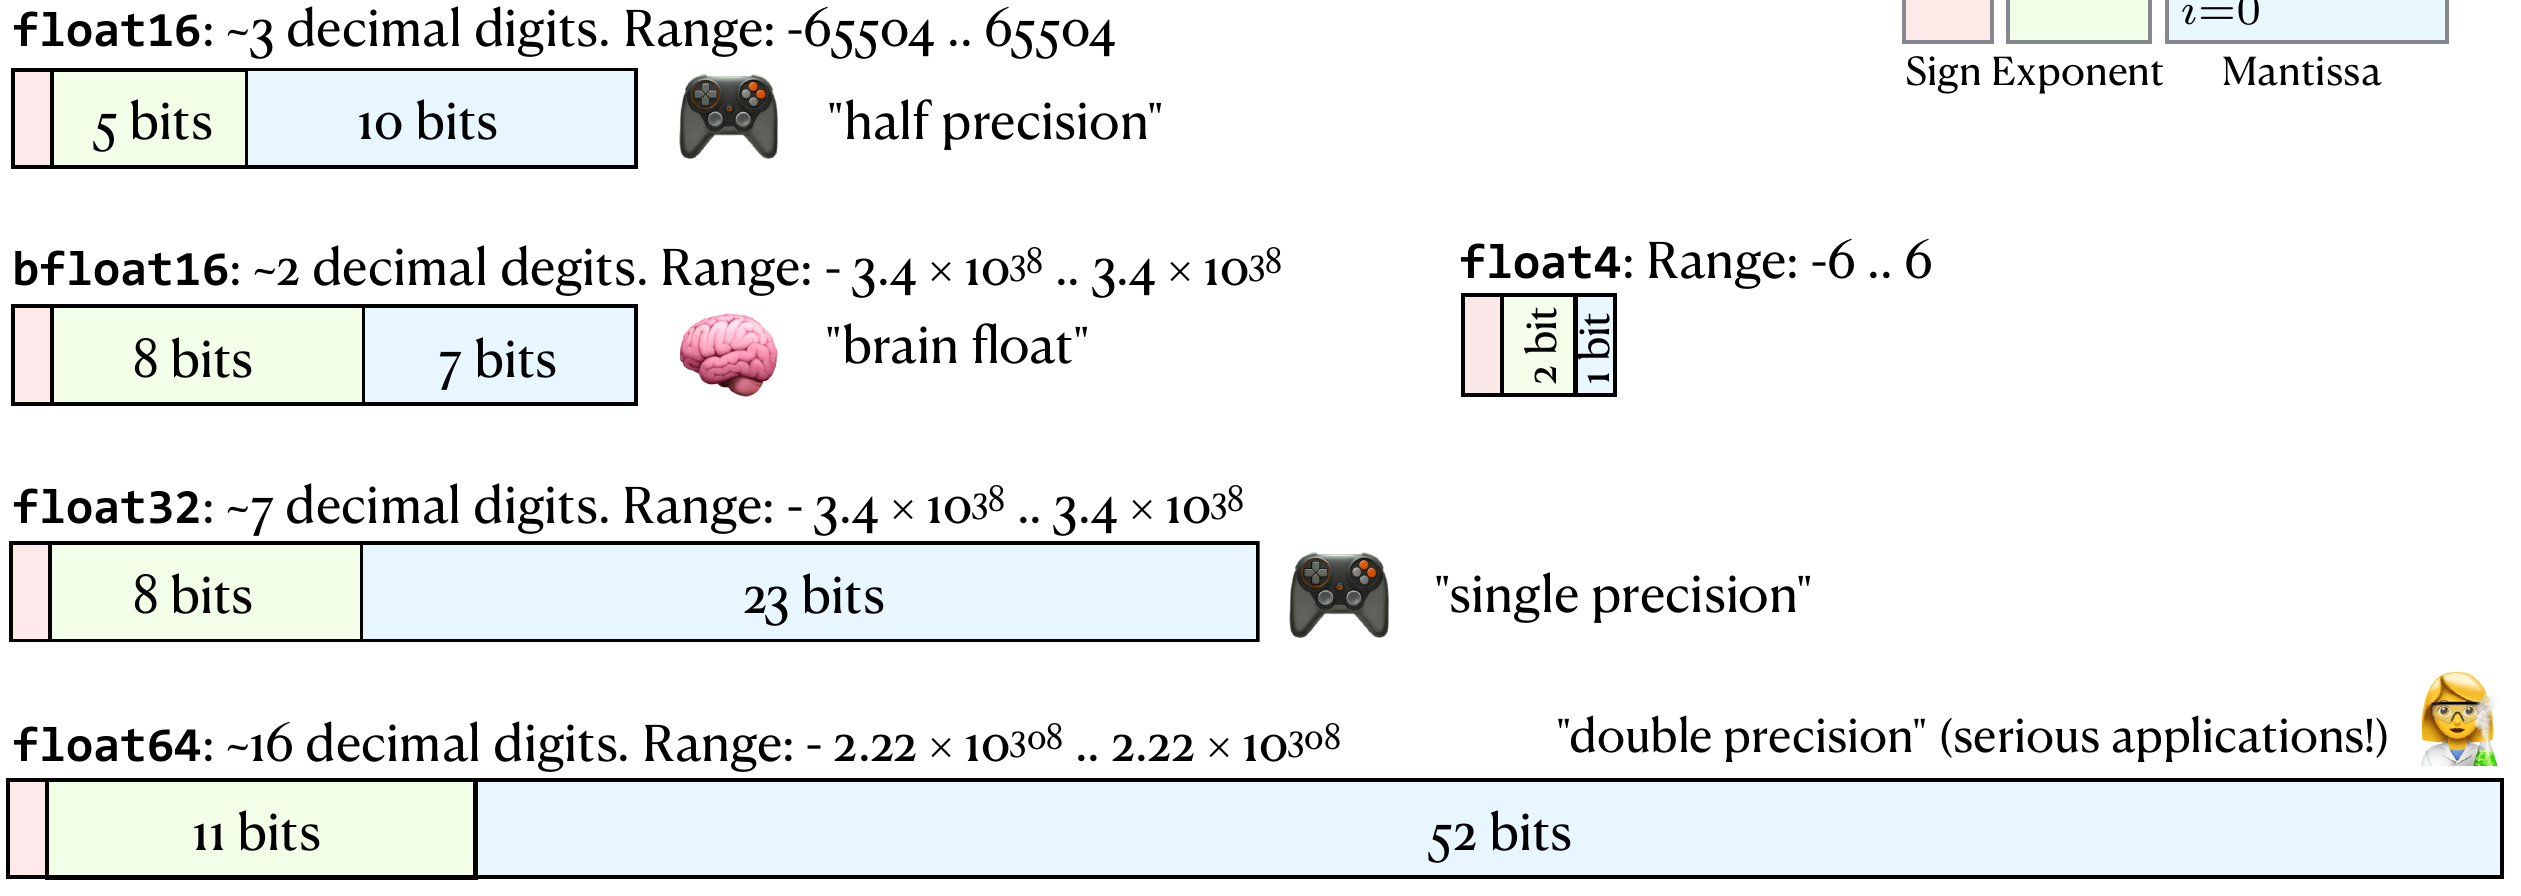
\includegraphics[width=\linewidth]{images/week01_01.png}
\end{center}
The density of representable numbers decreases with the magnitude; there is overflow beyond
the usable range and underflow near zero (``please don't memorize these numbers'').
\end{propbox}

\end{document}
